\section{Tuesday, February 14th: Input}
\subsection{Interface Critique}
\subsubsection{Dual-Screen Devices}
Why should we have these?
\begin{itemize}
    \item More screen space
\end{itemize}

Why haven't we seen more of these?
\begin{itemize}
    \item Moving parts $\implies$ Mechanical Complexity $\implies$ Fall apart quicker
    \item More expensive $\implies$ lower return on investment
    \item Aesthetics: there will likely be a crease in the middle
    \item Not much marginal benefit for the additional pixels
\end{itemize}

\myparagraph{Microsoft Research: Codex}
This dual screen tablet computer worked well with embedded sensors to detect when the 2 phones were detached.

\myparagraph{Microsoft Research: Courier}
Courier was a prototype concept by Microsoft for a dual-touchscreen tablet. The device was conceived as being a digital notebook, consisting of two 7-inch touchscreens hinged together like a book, and running a custom operating system built primarily around handwriting input and a notebook-like journal for storing notes, images, and clippings from web pages.

\subsection{Administravia: Midterm 1}
You can take the exam any time in-between 9am Tuesday Feb. 28th to 8:59am Wed, online. You have 90min to complete the exam once it has started (unless you have accommodations).

This will be done via bcourses as a quiz with a mix of MCQ (where you can choose multiple options -- select all that apply) and short answer + open-ended questions (can range from a sentence to a paragraph or two). \\
This gives you an opportunity to show your understanding in a variety of ways.

\subsubsection{Scope}
Lectures 1 to 11 and associated readings.

Make sure to know basic HTML/JS/CSS concepts + terminology from assignments and sections.

\subsection{Input Devices}
\subsubsection{Text Entry: Keystroke Devices}
We have 2 criteria:
\begin{enumerate}
    \item Fast
    \item Low error rate (accurate)
\end{enumerate}

There are good since we can (generally) expect where keys will be on the keyboard,
\myparagraph{DVORAK vs QWERTY}
QWERTY was made to prevent typewriter jams, and was transferred to computers for transfer learning benefits.

DVORAK is not popular as people are used to QWERTY and learning new tech is hard (per the Power law of practice).

\myparagraph{Mobile Difficulty}
If buttons are too small, you run into the ``fat-finger problem''

Solutions:
\begin{shaded}
Multi-tap mappings: Press a key multiple times to get a letter

Candybar Phones implemented this (T9 had recognition for $43556\to$ `hello'):
\begin{center}
    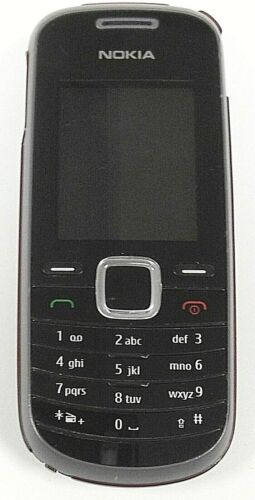
\includegraphics[scale=0.5]{lectures/wk5/img/candybar.jpg}
\end{center}
\end{shaded}

\myparagraph{Soft Keys}
Keys `f' and `j' have bumps on a computer keyboard but this tactile feedback information is lost on a touchscreen, which means you \textbf{have to} look at the screen to type.

\myparagraph{Drawing/Handwriting Recognition}
Why don't we use Drawing/Handwriting Recognition to input text?

Answer: it's slower than pressing keys

\myparagraph{Graffiti}
Custom alphabet with simplified symbols that are easier to recognize -- does not differentiate between lowercase and uppercase though.

\myparagraph{EdgeWrite}
Similar to Graffiti but Corner-based text input technique:
\begin{center}
    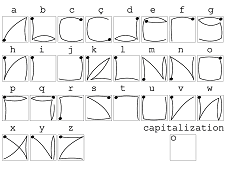
\includegraphics[scale=1]{lectures/wk5/img/edgewrite.png}
\end{center}

\myparagraph{Stroke writing}
You can also use backend algorithms to make this more accurate

\myparagraph{Speech Dictation}
This is $\sim$100 wpm. So why don't we always use this?
\begin{itemize}
    \item Privacy -- anyone nearby can hear
    \item Not socially acceptable -- to interrupt a quiet space with talking
    \item Can be hard to pickup \textit{only your} voice in a place with multiple people talking
    \item You have to know what you are going to say, ahead of time and that sort of `planning ahead' is more mentally demanding
    \begin{itemize}
        \item Editing previous words or even mistakes, is painful and adds more latency than doing the same operation on a keyboard.
    \end{itemize}
\end{itemize}

\subsection{Important Device Properties}
\subsubsection{Indirect vs Direct}
Direct: Input and Output space are unified (touchscreen)\\
Indirect: You're not pushing a button directly (mouse/trackpad/trackpoint)

\subsubsection{C:D Ratio}
For one unit of movement in physical space, how far does the 
cursor travel in display space?

Usually 1:1 for direct touch screen input.

\subsubsection{Device Acquisition Time}
Time between not using the device and starting to provide 
input

\subsection{Quadrature Encoding}
To use sensors for rotary encoding, you need $2$ bits of information:
\begin{enumerate}
    \item Which direction you are moving in
    \item How far you are moving in that direction
\end{enumerate}

\subsubsection{Optical Mice}
The physical mouse has hardware inside (a camera) which detects how much you have moved and which direction -- hundreds of times a second.

Fun fact: your mouse can be used as a (very bad) scanner.\\
It's not good as it doesn't have to be a repeatable proceeding device

\subsubsection{Trackpoint}
Lenovo Computers are known for having this red dot in the center.

\subsubsection{Resistive Touchscreens}
Cheap to manufacture  but only allows single-touch

\subsubsection{Capacitive Touchscreens}
Allow multi-touch

\begin{itemize}
    \item Direct input allows maximal screen space for mobile devices (ocular centrism).
    \item More degrees of freedom.
    \item ``Virtual input devices'' are adaptable.
    \item No extra pieces to lose or break (styli!)
\end{itemize}

\myparagraph{Exploit the edges}
Do not require users to explicitly click on some area/text. Instead allow the user to touch somewhere within some region an allow that to be sufficient to register an input click.
